\chapter{Polar Coordinates}

We have already seen how to plot a function with $(x,y)$ coordinates. For 
every $x$ that we put into a function, it returns a $y$. These pairs of 
coordinates tell us where on the $xy$-plane to graph the function. This 
coordinate system, where $x$ and $y$ are oriented horizontally and vertically, 
is called the \textit{Cartesian} coordinate system. It can be used to describe 
2D space, but it is not the only way. 

\begin{figure}[htbp]
\centering
    \begin{tikzpicture}
	\begin{axis}[xmin = 0, xmax = 3, ymin = 0, ymax = 3, axis lines = center, 
	xlabel = $x$, x label style = {anchor = north east}, ylabel = $y$, unit vector ratio*=1 1 1]
        \addplot[blue, mark=*] coordinates {(1, 2)};
        \draw[red, dashed](0,0) -- (1, 2);
        \addplot[red, domain = 0.31:0.84, samples = 200]{sqrt(0.5 - x^2)};
        \draw[red, -latex](0.35, 0.61) -- (0.3, 0.66);
        \node[black] at (2.1, 2.1) {$r = \sqrt{x^2 + y^2}$};
        \draw[black, -latex](1.5, 2) -- (0.75, 1.5);
        \node[] at (2.1, 0.5) {$\theta = \arctan{\frac{y}{x}}$};
        \node[] at (0.25, 0.15) {$\theta$};
        \draw[-latex](1.5, 0.5) -- (0.75, 0.15);
        \end{axis}
    \end{tikzpicture}
    \caption{The point $(1, 2)$ is $\sqrt{5}$ units from the origin and 
    approximately $1.107$ radians counterclockwise from horizontal}
    \label{fig:cartesian}
    \end{figure}

Instead of thinking about the horizontal and vertical position, we could think 
about distance from the origin and rotation about the origin. Take the 
Cartesian coordinate point $(1, 2)$ (see figure \ref{fig:cartesian}). How far is 
$(1,2)$ from the origin, $(0,0)$? We can create a right triangle, where the 
legs are parallel to the $x$ and $y$ axes. This means the leg lengths are 1 and 2, 
and we can use the Pythagorean theorem to find the length of the hypotenuse 
(which is the distance from the origin to the point):
$$c^2 = a^2 + b^2$$
$$c^2 = 1^2 + 2^2 = 1 + 4 = 5$$
$$c = \sqrt{5}$$

Therefore, the Cartesian point $(1, 2)$ is $\sqrt{5}$ units from the origin. 
This is not enough to find our point: there are infinite points that are 
$\sqrt{5}$ from the origin (see \ref{fig:circle}). To identify a particular point 
that is a distance of $\sqrt{5}$ from the origin, we also need an \textit{
angle of rotation}. By convention, angles are measured from the positive $x$-
axis. This means points on the positive $x$-axis have an angle of $\theta = 
0$, points on the positive $y$-axis have an angle of $\theta = \frac{\pi}{2}$, 
and so on. 

\begin{figure}[htbp]
\centering
    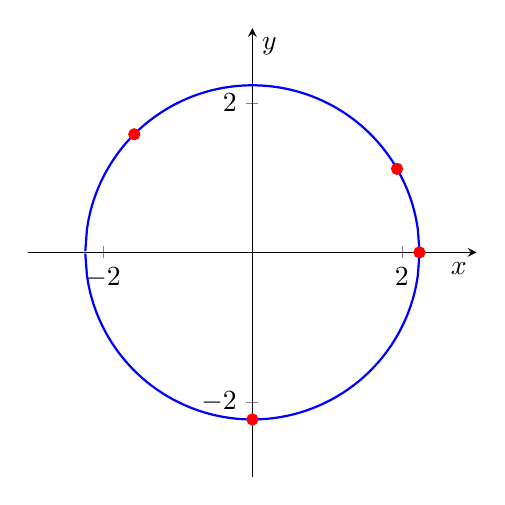
\begin{tikzpicture}
	\begin{axis}[xmin = -3, xmax = 3, ymin = -3, ymax = 3, axis lines = center, 
	xlabel = $x$, x label style = {anchor = north east}, ylabel = $y$, 
	unit vector ratio*=1 1 1]
        \addplot[blue, thick, domain = -2.236:2.236, samples = 200]{
        sqrt(5 - x^2)};
        \addplot[blue, thick, domain = -2.236:2.236, samples = 200]{
        -1*sqrt(5 - x^2)};
        \addplot[red, mark=*, only marks] coordinates {(2.236, 0) 
        (-1.581, 1.581) (1.936, 1.118) (0, -2.236)};
        \end{axis}
    \end{tikzpicture}
    \caption{There are infinite points $\sqrt{5}$ from the origin, represented 
    by the circle with a radius of $\sqrt{5}$ centered about the origin}
    \label{fig:circle}
    \end{figure}

We can use trigonometry to find the appropriate angle of rotation for our 
Cartesian point. There are many ways to do this, but using $\arctan$ is the 
most straightforward. Recall that:
$$\tan{\theta} = \frac{opposite}{adjacent}$$

That is, for a given angle in a right triangle, the tangent of that angle is 
given by the length of the opposite leg divided by the adjacent leg. In our 
case, the opposite leg is the vertical distance ($y$-value of the Cartesian 
point) and the adjacent leg is the horizontal distance ($x$-value of the 
Cartesian point), which means:
$$\tan{\theta} = \frac{2}{1}$$
$$\theta = \arctan{2} \approx 1.107\text{ radians}$$

\section{Plotting Polar Coordinate Points}
How do we plot polar coordinate points? Begin by locating the angle given by the second coordinate (remember, the angle is measured counterclockwise from the horizontal). Your point will lie somewhere on this line. Next, move outwards along the angle by the radius given by the first coordinate. 

\textbf{Example}: Plot the polar coordinate point $(2, \frac{\pi}{3})$. 

\textbf{Solution}: Begin by locating $\theta = \frac{\pi}{3}$ (see figure \ref{fig:plot1})

\begin{figure}[htbp]
\centering
	\begin{tikzpicture}
		\begin{polaraxis}[xtick = {0,0,deg((pi)/6),deg((2*pi)/6),deg((3*pi)/6),
	deg(4*pi)/6,deg((5*pi)/6), deg((6*pi)/6), deg((7*pi)/6), deg((8*pi)/6), 
	deg((9*pi)/6), deg((10*pi)/6), deg((11*pi)/6)}, xticklabels={,0,
	$\frac{\pi}{6}$,$\frac{\pi}{3}$,$\frac{\pi}{2}$,$\frac{2\pi}{3}$, 
	$\frac{5\pi}{6}$, $\pi$ ,$\frac{7\pi}{6}$, $\frac{4\pi}{3}$, 
	$\frac{3\pi}{2}$, $\frac{5\pi}{3}$, $\frac{11\pi}{6}$}, clip = false, ymax = 2.5]
			\draw[blue, dashed](0,0) -- (60, 2.5);
                \addplot[white, thick, domain = 0:360, samples = 300]{2.5};
		\end{polaraxis}
	\end{tikzpicture}
 \caption{$\theta = \frac{\pi}{3}$}
    \label{fig:plot1}
    \end{figure}

Then, move your finger or pencil along the line $\theta = \frac{\pi}{3}$ until you reach $r = 2$ (see figure \ref{fig:plot2}). 

\begin{figure}[htbp]
\centering
	\begin{tikzpicture}
		\begin{polaraxis}[xtick = {0,0,deg((pi)/6),deg((2*pi)/6),deg((3*pi)/6),
	deg(4*pi)/6,deg((5*pi)/6), deg((6*pi)/6), deg((7*pi)/6), deg((8*pi)/6), 
	deg((9*pi)/6), deg((10*pi)/6), deg((11*pi)/6)}, xticklabels={,0,
	$\frac{\pi}{6}$,$\frac{\pi}{3}$,$\frac{\pi}{2}$,$\frac{2\pi}{3}$, 
	$\frac{5\pi}{6}$, $\pi$ ,$\frac{7\pi}{6}$, $\frac{4\pi}{3}$, 
	$\frac{3\pi}{2}$, $\frac{5\pi}{3}$, $\frac{11\pi}{6}$}, clip = false, ymax = 2.5]
			\draw[blue, dashed](0,0) -- (60, 2.5);
                \addplot[blue, mark=*] coordinates {(60, 2)};
                \addplot[white, thick, domain = 0:360, samples = 300]{2.5};
		\end{polaraxis}
	\end{tikzpicture}
 	\caption{$(2, \frac{\pi}{3})$}
    \label{fig:plot2}
\end{figure}

\begin{Exercise}[label = polarplot]
Plot the following polar coordinate points on the provided polar axis (hint: negative angles are taken counterclockwise):
\begin{enumerate}
\item $(1, \pi)$
\item $(1.5, \frac{\pi}{2})$
\item $(1.5, -\frac{\pi}{6})$
\item $(2, \frac{3\pi}{4})$
\end{enumerate}
\centering
\begin{tikzpicture}
        \begin{polaraxis}[xtick = {0,0,deg((pi)/6),deg((2*pi)/6),deg((3*pi)/6),
	deg(4*pi)/6,deg((5*pi)/6), deg((6*pi)/6), deg((7*pi)/6), deg((8*pi)/6), 
	deg((9*pi)/6), deg((10*pi)/6), deg((11*pi)/6)}, xticklabels={,0,
	$\frac{\pi}{6}$,$\frac{\pi}{3}$,$\frac{\pi}{2}$,$\frac{2\pi}{3}$, 
	$\frac{5\pi}{6}$, $\pi$,$\frac{7\pi}{6}$, $\frac{4\pi}{3}$, 
	$\frac{3\pi}{2}$, $\frac{5\pi}{3}$, $\frac{11\pi}{6}$}, ymin = 0, ymax = 3, 
	clip = false]
	\addplot[white, thick, domain = 0:360, samples = 300]{3};
    \end{polaraxis}
    \end{tikzpicture}
\end{Exercise}

\begin{Answer}[ref = polarplot]
\begin{tikzpicture}
\centering
        \begin{polaraxis}[xtick = {0,0,deg((pi)/6),deg((2*pi)/6),deg((3*pi)/6),
	deg(4*pi)/6,deg((5*pi)/6), deg((6*pi)/6), deg((7*pi)/6), deg((8*pi)/6), 
	deg((9*pi)/6), deg((10*pi)/6), deg((11*pi)/6)}, xticklabels={,0,
	$\frac{\pi}{6}$,$\frac{\pi}{3}$,$\frac{\pi}{2}$,$\frac{2\pi}{3}$, 
	$\frac{5\pi}{6}$, $\pi$, $\frac{7\pi}{6}$, $\frac{4\pi}{3}$, 
	$\frac{3\pi}{2}$, $\frac{5\pi}{3}$, $\frac{11\pi}{6}$}, ymin = 0, ymax = 3, 
	clip = false]
 \addplot[white, thick, domain = 0:360, samples = 300]{3};
 \addplot[blue, mark=*, only marks] coordinates {(180, 1) (90, 1.5) (-30, 1.5) (135, 2)};
 \node[] at (180, 1.2) {$1$};
 \node[] at (90, 1.7) {$2$};
 \node[] at (-30, 1.7) {$3$};
 \node[] at (135, 2.2) {$4$};
    \end{polaraxis}
    \end{tikzpicture}
\end{Answer}

\section{Equivalent Points}
Unlike the Cartesian coordinate system, two different coordinates may lie at the same location. Consider the points $(1, \frac{\pi}{4})$ and $(-1, \frac{5\pi}{4})$ (see figure \ref{fig:eqpoints}). When a radius is negative, you move \textit{backwards} back over the origin, like a mirror image. 

\begin{figure}[htbp]
\centering
\begin{subfigure}{0.5\textwidth}
\centering
    \begin{tikzpicture}
	\begin{polaraxis}[xtick = {0,0,deg((pi)/6),deg((2*pi)/6),deg((3*pi)/6),
	deg(4*pi)/6,deg((5*pi)/6), deg((6*pi)/6), deg((7*pi)/6), deg((8*pi)/6), 
	deg((9*pi)/6), deg((10*pi)/6), deg((11*pi)/6)}, xticklabels={,0,
	$\frac{\pi}{6}$,$\frac{\pi}{3}$,$\frac{\pi}{2}$,$\frac{2\pi}{3}$, 
	$\frac{5\pi}{6}$, $\pi$ ,$\frac{7\pi}{6}$, $\frac{4\pi}{3}$, 
	$\frac{3\pi}{2}$, $\frac{5\pi}{3}$, $\frac{11\pi}{6}$}, clip = false, ymax = 1.5]
        \draw[blue, dashed](0,0) -- (45, 1.5);
        \draw[red, thick] (0,0) -- (45, 1);
        \addplot[red, mark=*] coordinates {(45, 1)};
        \addplot[blue, dashed, domain = 0:45]{0.75};
        \draw[black, latex-](15, 0.75) -- (-45, 0.5);
        \node[] at (-55, 0.55) {$\theta = \frac{\pi}{4}$};
        \draw[black, latex-](45, 0.5) -- (110, 1.25);
        \node[] at (110, 1.3) {$r = 1$};
        \addplot[white, thick, domain = 0:360, samples = 300]{1.5};
        \end{polaraxis}
    \end{tikzpicture}
\end{subfigure}
\begin{subfigure}{0.5\textwidth}
\centering
    \begin{tikzpicture}
        \begin{polaraxis}[xtick = {0,0,deg((pi)/6),deg((2*pi)/6),deg((3*pi)/6),
	deg(4*pi)/6,deg((5*pi)/6), deg((6*pi)/6), deg((7*pi)/6), deg((8*pi)/6), 
	deg((9*pi)/6), deg((10*pi)/6), deg((11*pi)/6)}, xticklabels={,0,
	$\frac{\pi}{6}$,$\frac{\pi}{3}$,$\frac{\pi}{2}$,$\frac{2\pi}{3}$, 
	$\frac{5\pi}{6}$, $\pi$ ,$\frac{7\pi}{6}$, $\frac{4\pi}{3}$, 
	$\frac{3\pi}{2}$, $\frac{5\pi}{3}$, $\frac{11\pi}{6}$}, clip = false, ymax = 1.5]
        \draw[blue, dashed](0,0) -- (225, 1.5);
        \draw[red, thick] (0,0) -- (45, 1);
        \addplot[red, mark=*] coordinates {(45, 1)};
        \draw[red, dashed] (0,0) -- (225, 1);
        \addplot[blue, dashed, domain = 0:225]{0.75};
        \draw[black, -latex](127, 1.15) -- (115, 0.75);
        \draw[black, -latex](-95, 1.25) -- (225, 0.5);
        \node[] at (-95, 1.28) {$r = 1$};
        \draw[black, -latex] (-45, 1) -- (45, 0.35);
        \node[] at (-45, 1.1) {$r = -1$};
        \addplot[white, thick, domain = 0:360, samples = 300]{1.5};
        \node[] at (135, 1.3) {$\theta = \frac{5\pi}{4}$};
        \end{polaraxis}
    \end{tikzpicture}
\end{subfigure}
    \caption{The polar coordinates points $(1, \frac{\pi}{4})$ and $(-1, \frac{5\pi}{4})$ are the same location on a polar axis}
    \label{fig:eqpoints}
    \end{figure}

\section{Changing coordinate systems}

\subsection{Cartesian to Polar}
From the example above, you should see that a given Cartesian coordinate, 
$(x,y)$, can also be expressed as a polar coordinate, $(r, \theta)$, where $r$ 
is the distance from the origin and $\theta$ is the angle of rotation from the 
horizontal. (Note: Polar functions are generally given as $r$ defined in terms 
of $\theta$, which means the \textit{dependent} variable is listed first in 
the coordinate pair, unlike Cartesian coodinates.) Additionally, 
$$r = \sqrt{x^2 + y^2}$$
$$\theta = \arctan{\frac{y}{x}}$$

\textbf{Example}: Express the Cartesian point $(-3, 4)$ in polar coordinates. 

\textbf{Solution}: Taking $x = -3$ and $y = 4$, we find that:
$$r = \sqrt{(-3)^2 + 4^2} = \sqrt{9 + 16} = \sqrt{25} = 5$$

We follow the convention of only taking the positive solution to the square 
root. Finding $\theta$:
$$\theta = \arctan{\frac{4}{-3}}$$

When you evaluate the $\arctan$ with a calculator, you are likely to get back 
$\theta = -0.928$. Recall that $tan{\theta} = \tan{\theta \pm n\pi}$, where $n$ 
is an integer. We know our Cartesian point, $(-3, 4)$, is in the II quadrant, 
while the angle $-0.928$ radians would fall in the IV quadrant. So, clearly, 
$-0.928$ radians is not correct. Most calculators restrict the output of 
$\arctan$ to angles between $-\frac{\pi}{2}$ and $\frac{\pi}{2}$, because 
there are actually multiple angles where $\tan{\theta} = -\frac{4}{3}$. Since 
$\tan{\theta} = \tan{\theta \pm n \pi}$, we also know that:
$$\arctan{-\frac{4}{3}} = -0.928 \pm n \pi$$

Another possible $\theta$ is $-0.928 + \pi \approx 2.214$, which does fall 
in the appropriate quadrant. This means the polar coordinates $(5, 2.214)$ are the 
same as the Cartesian coordinates $(-3, 4)$. \textit{Note:} It is standard 
practice to express angles in radians, and not degrees, when using polar 
coordinates. 

\subsection{Polar to Cartesian}
We can also leverage our knowledge of right triangles to convert polar 
coordinates to Cartesian coordinates. Take the polar coordinate $(2, 
\frac{\pi}{4})$ (see figure \ref{fig:polar_to_cart}). We can draw a right 
triangle with legs parallel to the $x$ and $y$ axes (not shown in the figure) 
and a hypotenuse that goes from the origin to the polar coordinate $(2, \frac{
\pi}{4})$. 

\begin{figure}[htbp]
\centering
    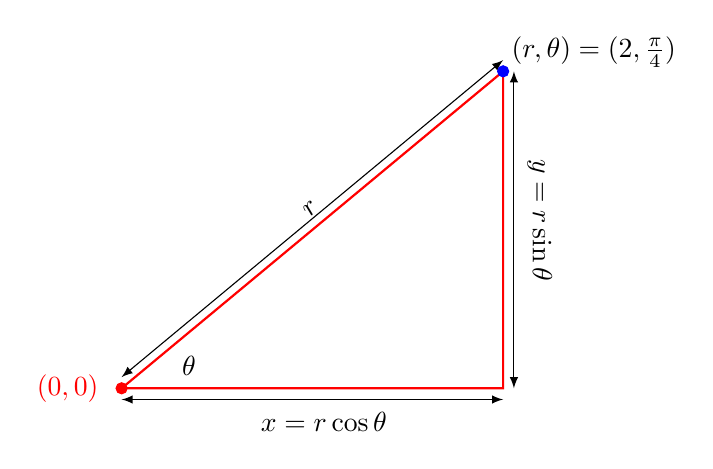
\begin{tikzpicture}
	\begin{axis}[axis lines = none, xmin = 0, xmax = 2, ymin = 0, ymax = 2, 
	clip = false]
        \addplot[blue, mark=*] coordinates {(1.414, 1.414)};
        \addplot[red, mark=*] coordinates {(0,0)};
        \draw[red, thick] (0,0) -- (1.414, 0) -- (1.414, 1.414) -- cycle;
        \node[] at (1.75, 1.5) {$(r, \theta) = (2, \frac{\pi}{4})$};
        \node[] at (0.25, 0.1) {$\theta$};
        \draw[latex - latex] (0, 0.05) -- (1.414, 1.464);
        \node[rotate = 45] at (0.7, 0.8) {$r$};
        \draw[latex - latex] (1.454, 0) -- (1.454, 1.414);
        \node[rotate = -90] at (1.55, 0.75) {$y = r\sin{\theta}$};
        \draw[latex - latex] (0,-0.05) -- (1.414, -0.05);
        \node[] at (0.75, -0.15) {$x = r\cos{\theta}$};
        \node[red] at (-0.2, 0) {$(0,0)$};
        \end{axis}
    \end{tikzpicture}  
    \caption{To convert from polar to Cartesian coordinates, use the identities 
    $x = r\cos{\theta}$ and $y = r\sin{\theta}$}
    \label{fig:polar_to_cart}
    \end{figure}

Recall from trigonometry that:
$$\sin{\theta} = \frac{\text{opposite leg}}{\text{hypotenuse}}$$
We know that the hypotenuse of this triangle has a length of $r$. The opposite 
leg is vertical and is the same length as the distance of the polar coordinate 
from the $x$-axis. Therefore, the length of the vertical leg represents the 
$y$ value of that same polar coordinate if it were expressed in Cartesian 
coordinates. So, we can say that:
$$\sin{\theta} = \frac{y}{r}$$
And therefore:
$$y = r\sin{\theta}$$

By a similar process, we also see that:
$$x = r\cos{\theta}$$

This is easy to visualize and understand for $0 \leq \theta \leq \frac{\pi}{
2}$, but it also holds for other values of $\theta$. 

\textbf{Example}: Express the polar coordinate $(\frac{3}{2}, \frac{2\pi}{3})$ 
in Cartesian coordinates.

\textbf{Solution}: From the polar coordinate, we see that $\theta = \frac{2\pi
}{3}$ and $r = \frac{3}{2}$. Therefore:
$$x = r\cos{\theta} = \frac{3}{2} \cdot \cos{\frac{2\pi}{3}} = \frac{3}{2} 
\cdot -\frac{1}{2} = -\frac{3}{4}$$
$$y = r\sin{\theta} = \frac{3}{2} \cdot \sin{\frac{2\pi}{3}} = \frac{3}{2} 
\cdot \frac{\sqrt{3}}{2} = \frac{3\sqrt{3}}{4}$$

The Cartesian coordinate $(-\frac{3}{4}, \frac{3\sqrt{3}}{4})$ has the 
same location as the given polar coordinate. 

\begin{Exercise}[label = convert1]
Convert the following polar coordinates to Cartesian coordinates: 
\begin{enumerate}
\item $(2, \frac{3\pi}{2})$
\item $(\sqrt{2}, \frac{3\pi}{4})$
\item $(3, -\frac{\pi}{4})$
\item $(-3, -\frac{\pi}{3})$
\item $(2, -\frac{\pi}{2})$
\end{enumerate}
\end{Exercise}

\begin{Answer}[ref = convert1]
\begin{enumerate}
\item $(0, -2)$. $x = 2 \cdot \cos{\frac{3\pi}{2}} = 2 \cdot 0 = 0$ and $y = 2 
\cdot \sin{\frac{3\pi}{2}} = 2 \cdot -1 = -2$.
\item $(-1,1)$. $x = \sqrt{2} \cdot \cos{\frac{3\pi}{4}} = \sqrt{2} \cdot - 
\frac{\sqrt{2}}{2} = \frac{2}{2} = -1$ and $y = \sqrt{2} \cdot \sin{\frac{3
\pi}{4}} = \sqrt{2} \cdot \frac{\sqrt{2}}{2} = \frac{2}{2} = 1$. 
\item $(\frac{3\sqrt{2}}{2}, -\frac{3\sqrt{2}}{2})$. $x = 3 \cdot \cos{-\frac{
\pi}{4}} = 3 \cdot \frac{\sqrt{2}}{2} = \frac{3\sqrt{2}}{2}$ and $y = 3 \cdot 
\sin{-\frac{\pi}{4}} = 3 \cdot -\frac{\sqrt{2}}{2} = -\frac{3\sqrt{2}}{2}$.
\item $(-\frac{3}{2}, -\frac{3\sqrt{3}}{2})$. $x = (-3) \cdot \cos{\frac{\pi}{3
}} = (-3) \cdot \frac{1}{2} = -\frac{3}{2}$ and $y = (-3) \cdot \sin{\frac{\pi
}{3}} = (-3) \cdot \frac{\sqrt{3}}{2} = - \frac{3\sqrt{3}}{2}$.
\item $(0, -2)$. $x = 2 \cdot \cos{-\frac{pi}{2}} = 2 \cdot 0 = 0$ and $y = 2 
\cdot \sin{-\frac{\pi}{2}} = 2 \cdot -1 = -2$. 
\end{enumerate}
\end{Answer}

\begin{Exercise}[label = convert2]
Convert the following Cartesian coordinates to polar coordinates. Restrict 
$\theta$ to $0 \leq \theta < 2\pi$. 
\begin{enumerate}
\item $(-4, 4)$
\item $(3, 3\sqrt{3})$
\item $(\sqrt{3}, -1)$
\item $(-6, 0)$
\item $(-2, -2)$
\end{enumerate}
\end{Exercise}

\begin{Answer}[ref = convert2]
\begin{enumerate}
\item $(4\sqrt{2}, \frac{3\pi}{4})$. $r = \sqrt{x^2 + y^2} = \sqrt{32} = 4
\sqrt{2}$. $\arctan{\frac{y}{x}} = \arctan{\frac{4}{-4}} = \arctan{-1} = -
\frac{\pi}{4} + n\pi$. We take $\theta = \frac{3\pi}{4}$ to satisfy the domain 
restriction and be in the correct quadrant. 
\item $(6, \frac{\pi}{3})$. $r = \sqrt{3^2 + \left( 3\sqrt{3} \right)^2} = 
\sqrt{9 + 27} = \sqrt{36} = 6$. $arctan{\frac{3\sqrt{3}}{3}} = \arctan{\sqrt{
3}} = \frac{\pi}{3} + n\pi$. We take $\theta = \frac{\pi}{3}$ to satisfy the 
domain restriction and be in the correct quadrant. 
\item $(2,\frac{11\pi}{6})$. $r = \sqrt{\sqrt{3}^2 + (-1)^2} = \sqrt{3 + 1} = 
2$. $\arctan{\frac{-1}{\sqrt{3}}} = -\frac{\pi}{6} + n\pi$. We take $\theta = 
\frac{11\pi}{6}$ to satisfy the domain restriction and have the point in the 
correct quadrant. 
\item $(6, \pi)$. $r = \sqrt{(-6)^2 + 0^2} = 6$. $\arctan{\frac{0}{-6}} = \pi 
+ n\pi$. We take $\theta = \pi$ to satisfy the domain restriction. 
\item $(2\sqrt{2}, \frac{5\pi}{4})$. $r = \sqrt{(-2)^2 + (-2)^2} = \sqrt{8} = 
2\sqrt{2}$. $\arctan{\frac{-2}{-2}} = \arctan{1} = \frac{\pi}{4} + n\pi$. We 
take $\theta = \frac{5\pi}{4}$ to satisfy the domain restriction and be in the 
correct quadrant. 
\end{enumerate}
\end{Answer}



\section{Circles in Polar Coordinates}
Many conic sections, including circles, are simpler to express as polar 
functions than as Cartesian functions. Consider a circle with a radius of $2$ 
centered about the origin. The polar function for this is $r = 2$ for all 
$\theta$. Let's write a Cartesian function for the same circle. 

We know that for every point on the circle, the distance to the origin is $2$. 
This means that, by the Pythagorean theorem, 
$$r^2 = x^2 + y^2$$.

(see figure \ref{fig:circle2})

\begin{figure}[htbp]
\centering
    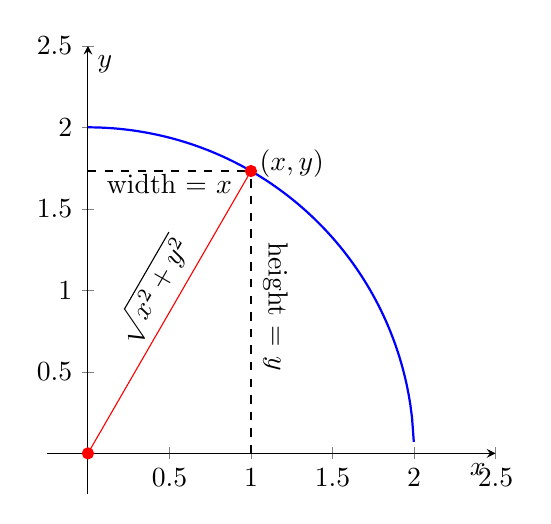
\begin{tikzpicture}
	\begin{axis}[xmin = -0.25, xmax = 2.5, ymin = -0.25, ymax = 2.5, axis lines 
	= center, xlabel = $x$, x label style = {anchor = north east}, ylabel = $y$, 
	unit vector ratio*=1 1 1]
        \addplot[blue, thick, domain = 0:2.15, samples = 200]{
        sqrt(4 - x^2)};
        \addplot[red, mark=*] coordinates {(0,0) (1, 1.732)};
        \node[black] at (1.25, 1.78) {$(x, y)$};
        \draw[black, dashed] (1, 0) -- (1, 1.732);
        \draw[black, dashed] (0, 1.732) -- (1, 1.732);
        \node[black] at (0.5, 1.65) {width = $x$};
        \node[black, rotate = -90] at (1.15, 0.9) {height = $y$};
        \node[rotate = 60] at (0.4,1) {$\sqrt{x^2 + y^2}$};
        \end{axis}
    \end{tikzpicture}
    \caption{All $(x,y)$ pairs on the circle are the same distance from the origin}
    \label{fig:circle2}
    \end{figure}
    
We can solve this equation for $y$, given that $r = 2$ (in this case):
$$y = \pm \sqrt{2^2 - x^2}$$

Notice that this is really two equations: $y = \sqrt{2^2 - x^2}$ and $y = -\sqrt{
2^2 - x^2}$. This is more complex than the polar equation, $r = 2$. 

As seen above, the equation of a circle with radius $R$ centered on the origin 
is simply $r = R$ in polar coordinates. What if we want a circle centered 
somewhere else? Polar coordinates are best when a circle is bisected by the 
$x$ or $y$ axis. Consider the polar equation $r = 3 \sin{\theta}$. Let's use a 
table to find some points and plot the function:

\begin{center}
\begin{tabular}{|c|c|}\hline
$\theta$ & $r = 3 \sin{\theta}$\\\hline
$0$ & $0$\\\hline
$\frac{\pi}{6}$ & $\frac{3}{2}$\\\hline
$\frac{\pi}{4}$ & $\frac{3\sqrt{2}}{2}$\\\hline
$\frac{\pi}{3}$ & $\frac{3\sqrt{3}}{2}$\\\hline
$\frac{\pi}{2}$ & $3$\\\hline
$\frac{2\pi}{3}$ & $\frac{3\sqrt{3}}{2}$\\\hline
$\frac{3\pi}{4}$ & $\frac{3\sqrt{2}}{2}$\\\hline
$\frac{5\pi}{6}$ & $\frac{3}{2}$\\\hline
$\pi$ & $0$\\\hline
\end{tabular}
\end{center}


Here is how those points look plotted (see figures \ref{fig:sinecircle} and 
\ref{fig:polarsine}):

\begin{figure}[htbp]
\centering
\begin{subfigure}{0.5\textwidth}
\centering
    \begin{tikzpicture}
	\begin{axis}[xmin = -3.25, xmax = 3.25, ymin = -0.25, ymax = 3.25, 
	axis lines = center, xlabel = $x$, x label style = {anchor = north east}, 
	ylabel = $y$, unit vector ratio*=1 1 1]
        \addplot[red, mark=*, only marks] coordinates {(0,0) (1.299, 0.75) 
        (1.5, 1.5) (1.299, 2.25) (0, 3) (-1.299, 2.25) (-1.5, 1.5) 
        (-1.299, 0.75)};
        \end{axis}
    \end{tikzpicture}
\end{subfigure}
\begin{subfigure}{0.5\textwidth}
\centering
    \begin{tikzpicture}
        \begin{polaraxis}[xtick = {0,0,deg((pi)/6),deg((2*pi)/6),deg((3*pi)/6),
	deg(4*pi)/6,deg((5*pi)/6), deg((6*pi)/6)}, xticklabels={,0,
	$\frac{\pi}{6}$,$\frac{\pi}{3}$,$\frac{\pi}{2}$,$\frac{2\pi}{3}$, 
	$\frac{5\pi}{6}$, $\pi$}, xmin = 0, xmax = 180, ymax = 3.25, clip = false]
        \addplot[red, mark=*, only marks] coordinates {(0, 0) (30, 3/2) (45, 2.121) (60, 2.598) (90, 3) (120, 2.598) (135, 2.121) (150, 3/2) (180, 0)};
        \addplot[white, thick, domain = 0:180, samples = 300]{3.25};
        \end{polaraxis}
    \end{tikzpicture}
\end{subfigure}
    \caption{Several points for $r = 3\sin{\theta}$ plotted on Cartesian and polar coordinate systems}
    \label{fig:sinecircle}
    \end{figure}

\begin{figure}[htbp]
    \centering
    \begin{tikzpicture}
        \begin{polaraxis}[xtick = {0,0,deg((pi)/6),deg((2*pi)/6),deg((3*pi)/6),
	deg(4*pi)/6,deg((5*pi)/6), deg((6*pi)/6), deg((7*pi)/6), deg((8*pi)/6), 
	deg((9*pi)/6), deg((10*pi)/6), deg((11*pi)/6)}, xticklabels={,0,
	$\frac{\pi}{6}$,$\frac{\pi}{3}$,$\frac{\pi}{2}$,$\frac{2\pi}{3}$, 
	$\frac{5\pi}{6}$, $\pi$, $\frac{7\pi}{6}$, $\frac{4\pi}{3}$, 
	$\frac{3\pi}{2}$, $\frac{5\pi}{3}$, $\frac{11\pi}{6}$}, clip = false, ymax = 3.3]
        \addplot[blue, thick, domain = 0:180, samples = 200]{3*sin(x)};
        \addplot[white, thick, domain = 0:360, samples = 300]{3.3};
    \end{polaraxis}
    \end{tikzpicture}
    \caption{$r = 3\sin{\theta}$ plotted on a polar coordinate system}
    \label{fig:polarsine}
\end{figure}

So, the polar equation $r = 3 \sin{\theta}$ gives a circle with radius $\frac{3
}{2}$ centered at $(0, \frac{3}{2})$. 

\textbf{Example}: Describe the graph of $r = \cos{\theta}$. Feel free to make 
a rough plot on the blank polar axis below:

\begin{center}
\begin{tikzpicture}

        \begin{polaraxis}[xtick = {0,0,deg((pi)/6),deg((2*pi)/6),deg((3*pi)/6),
	deg(4*pi)/6,deg((5*pi)/6), deg((6*pi)/6), deg((7*pi)/6), deg((8*pi)/6), 
	deg((9*pi)/6), deg((10*pi)/6), deg((11*pi)/6)}, xticklabels={,0,
	$\frac{\pi}{6}$,$\frac{\pi}{3}$,$\frac{\pi}{2}$,$\frac{2\pi}{3}$, 
	$\frac{5\pi}{6}$,$\pi$ ,$\frac{7\pi}{6}$, $\frac{4\pi}{3}$, 
	$\frac{3\pi}{2}$, $\frac{5\pi}{3}$, $\frac{11\pi}{6}$}, ymin = 0, ymax = 1.5, 
	clip = false]
	\addplot[white, thick, domain = 0:360, samples = 300]{1.5};
    \node[black] at (2.5, 1.49) {.};
    \end{polaraxis}
    \end{tikzpicture}
\end{center}

    
\textbf{Solution}: This plot will look like a circle of radius 0.5 centered at 
$(0.5, 0)$ (in polar coordinates). 

\begin{center}
\begin{tikzpicture}
        \begin{polaraxis}[xtick = {0,0,deg((pi)/6),deg((2*pi)/6),deg((3*pi)/6),
	deg(4*pi)/6,deg((5*pi)/6), deg((6*pi)/6), deg((7*pi)/6), deg((8*pi)/6), 
	deg((9*pi)/6), deg((10*pi)/6), deg((11*pi)/6)}, xticklabels={,0,
	$\frac{\pi}{6}$,$\frac{\pi}{3}$,$\frac{\pi}{2}$,$\frac{2\pi}{3}$, 
	$\frac{5\pi}{6}$, $\pi$, $\frac{7\pi}{6}$, $\frac{4\pi}{3}$, 
	$\frac{3\pi}{2}$, $\frac{5\pi}{3}$, $\frac{11\pi}{6}$}, ymin = 0, ymax = 1.5, 
	clip = false]
	\addplot[white, thick, domain = 0:360, samples = 300]{1.5};
    \addplot[blue, thick, domain = 0:180, samples = 200]{cos(x)};
    \node[black] at (2.5, 1.49) {.};
    \end{polaraxis}
    \end{tikzpicture}
\end{center}


\begin{Exercise}[label = circles]
Sketch the following polar functions on the provided polar axis for $0 \leq 
\theta < 2\pi$:
\begin{enumerate}
\item $r = 3$
\item $\theta = \pi$
\item $r = 2\cos{\frac{\theta}{2}}$
\item $r = -4\sin{\theta}$
\item $r = \theta$
\end{enumerate}
\centering
\begin{tikzpicture}
        \begin{polaraxis}[xtick = {0,0,deg((pi)/6),deg((2*pi)/6),deg((3*pi)/6),
	deg(4*pi)/6,deg((5*pi)/6), deg((6*pi)/6), deg((7*pi)/6), deg((8*pi)/6), 
	deg((9*pi)/6), deg((10*pi)/6), deg((11*pi)/6)}, xticklabels={,0,
	$\frac{\pi}{6}$,$\frac{\pi}{3}$,$\frac{\pi}{2}$,$\frac{2\pi}{3}$, 
	$\frac{5\pi}{6}$, $\pi$, $\frac{7\pi}{6}$, $\frac{4\pi}{3}$, 
	$\frac{3\pi}{2}$, $\frac{5\pi}{3}$, $\frac{11\pi}{6}$}, ymin = 0, ymax = 5, 
	clip = false]
	\addplot[white, thick, domain = 0:360, samples = 300]{5};
    \end{polaraxis}
    \end{tikzpicture}
\end{Exercise}

\begin{Answer}[ref = circles2]
\begin{enumerate}
\item $r = 3$

\begin{center}
\begin{tikzpicture}
        \begin{polaraxis}[xtick = {0,0,deg((pi)/6),deg((2*pi)/6),deg((3*pi)/6),
	deg(4*pi)/6,deg((5*pi)/6), deg((6*pi)/6), deg((7*pi)/6), deg((8*pi)/6), 
	deg((9*pi)/6), deg((10*pi)/6), deg((11*pi)/6)}, xticklabels={,0,
	$\frac{\pi}{6}$,$\frac{\pi}{3}$,$\frac{\pi}{2}$,$\frac{2\pi}{3}$, 
	$\frac{5\pi}{6}$, $\pi$, $\frac{7\pi}{6}$, $\frac{4\pi}{3}$, 
	$\frac{3\pi}{2}$, $\frac{5\pi}{3}$, $\frac{11\pi}{6}$}, ymin = 0, ymax = 5, 
	clip = false]
    \addplot[blue, thick, domain = 0:360, samples = 200]{3};
    \addplot[white, thick, domain = 0:360, samples = 300]{5};
    \end{polaraxis}
    \end{tikzpicture}
\end{center}

    
\item $\theta = \pi$ Because $r$ includes all real numbers, negative $r$ is possible and the 
line $\theta = \pi$ extends in both directions

\begin{center}
\begin{tikzpicture}
        \begin{polaraxis}[xtick = {0,0,deg((pi)/6),deg((2*pi)/6),deg((3*pi)/6),
	deg(4*pi)/6,deg((5*pi)/6), deg((6*pi)/6), deg((7*pi)/6), deg((8*pi)/6), 
	deg((9*pi)/6), deg((10*pi)/6), deg((11*pi)/6)}, xticklabels={,0,
	$\frac{\pi}{6}$,$\frac{\pi}{3}$,$\frac{\pi}{2}$,$\frac{2\pi}{3}$, 
	$\frac{5\pi}{6}$, $\pi$, $\frac{7\pi}{6}$, $\frac{4\pi}{3}$, 
	$\frac{3\pi}{2}$, $\frac{5\pi}{3}$, $\frac{11\pi}{6}$}, ymin = 0, ymax = 5, 
	clip = false]
    \draw[blue, thick, latex-latex] (0, 5) -- (180,5);
    \addplot[white, thick, domain = 0:360, samples = 300]{5};
    \end{polaraxis}
    \end{tikzpicture}
\end{center}


\item $r = 2\cos{\frac{\theta}{2}}$

\begin{center}
\begin{tikzpicture}
        \begin{polaraxis}[xtick = {0,0,deg((pi)/6),deg((2*pi)/6),deg((3*pi)/6),
	deg(4*pi)/6,deg((5*pi)/6), deg((6*pi)/6), deg((7*pi)/6), deg((8*pi)/6), 
	deg((9*pi)/6), deg((10*pi)/6), deg((11*pi)/6)}, xticklabels={,0,
	$\frac{\pi}{6}$,$\frac{\pi}{3}$,$\frac{\pi}{2}$,$\frac{2\pi}{3}$, 
	$\frac{5\pi}{6}$, $\pi$,$\frac{7\pi}{6}$, $\frac{4\pi}{3}$, 
	$\frac{3\pi}{2}$, $\frac{5\pi}{3}$, $\frac{11\pi}{6}$}, ymin = 0, ymax = 5, 
	clip = false]
    \addplot[blue, thick, domain = 0:360, samples = 200]{2*cos(x/2)};
    \addplot[white, thick, domain = 0:360, samples = 300]{5};
    \end{polaraxis}
    \end{tikzpicture}
\end{center}

    
\item $r = -4\sin{\theta}$

\begin{center}
\begin{tikzpicture}
        \begin{polaraxis}[xtick = {0,0,deg((pi)/6),deg((2*pi)/6),deg((3*pi)/6),
	deg(4*pi)/6,deg((5*pi)/6), deg((6*pi)/6), deg((7*pi)/6), deg((8*pi)/6), 
	deg((9*pi)/6), deg((10*pi)/6), deg((11*pi)/6)}, xticklabels={,0,
	$\frac{\pi}{6}$,$\frac{\pi}{3}$,$\frac{\pi}{2}$,$\frac{2\pi}{3}$, 
	$\frac{5\pi}{6}$, $\pi$, $\frac{7\pi}{6}$, $\frac{4\pi}{3}$, 
	$\frac{3\pi}{2}$, $\frac{5\pi}{3}$, $\frac{11\pi}{6}$}, ymin = 0, ymax = 5, 
	clip = false]
    \addplot[blue, thick, domain = 0:360, samples = 200]{-4*sin(x)};
    \addplot[white, thick, domain = 0:360, samples = 300]{5};
    \end{polaraxis}
    \end{tikzpicture}
\end{center}

    
\item $r = \theta$ (The spiral continues, but is beyond the boundary of the graph)

\begin{center}
\begin{tikzpicture}
        \begin{polaraxis}[xtick = {0,0,deg((pi)/6),deg((2*pi)/6),deg((3*pi)/6),
	deg(4*pi)/6,deg((5*pi)/6), deg((6*pi)/6), deg((7*pi)/6), deg((8*pi)/6), 
	deg((9*pi)/6), deg((10*pi)/6), deg((11*pi)/6)}, xticklabels={,0,
	$\frac{\pi}{6}$,$\frac{\pi}{3}$,$\frac{\pi}{2}$,$\frac{2\pi}{3}$, 
	$\frac{5\pi}{6}$, $\pi$, $\frac{7\pi}{6}$, $\frac{4\pi}{3}$, 
	$\frac{3\pi}{2}$, $\frac{5\pi}{3}$, $\frac{11\pi}{6}$}, ymin = 0, ymax = 5, 
	clip = false]
    \addplot[blue, thick, domain = 0:286, samples = 200]{x*(2*pi)/360};
    \addplot[white, thick, domain = 0:360, samples = 300]{5};
    \end{polaraxis}
    \end{tikzpicture}
\end{center}

\end{enumerate}
\end{Answer}

% do we want to include a section about petals and flowers in polar coordinates? would be good for polar integration prep